\documentclass[10pt]{article}

\usepackage[utf8]{inputenc}
\usepackage[french]{babel}
\usepackage{amsmath}
\usepackage{amsfonts}
\usepackage{amssymb}
\usepackage{graphicx}
\usepackage{parskip}
\usepackage{multicol}


\newcommand{\NP}{\text{NP}}

\begin{document}


\title{IFT2105 - Devoir 3}
\date{Novembre 2010}
\author{Vincent Foley-Bourgon (FOLV08078309)}
\maketitle

\section{Question 1}

\emph{Montrer que L est NP-complet où:}
\[
L = \{ G : G \text{ est un graphe de $n$ noeuds ayant une clique de
  taille au moins $n/2$} \}
\]

Un langage $L$ est NP-complet si:
\begin{enumerate}
  \item $L \in \NP$
  \item $L$ est NP-difficile
\end{enumerate}

\subsection{$L \in \NP$}

$L$ appartient à la classe NP s'il existe une machine de Turing
fonctionnant en temps polynomial qui, étant donné un certificat $C$,
\emph{vérifie} si un mot appartient à $L$.

Prenons comme certificat l'ensemble des noeuds formant la clique; il
est possible de vérifier en temps polynomial que ces noeuds forment un
graphe complet:

\begin{verbatim}
Verificateur(G, C):
  si |G|/2 > |C|:
    retourner faux

  pour chaque noeud dans C:
    pour chaque autre-noeud dans C \ {noeud}:
      si noeud et autre-noeud ne sont pas voisins:
        retourner faux
      fin si
    fin pour
  fin pour
  retourner vrai
fin
\end{verbatim}

\emph{Verificateur} fonctionne en $O(n^2)$, donc $L \in \NP$.

\subsection{$L$ est NP-difficile}

$L$ est NP-difficile si $L$ est au moins aussi difficile que tous les
autres langages dans NP.  Écrit de façon mathématique, pour tout
langage $K$ de NP, il existe une fonction $f$ qui permet de réduire
$K$ à $L$ en temps polynomial (noté $K \le_p L$) et donc $w \in K \iff
f(w) \in L$.

\subsubsection{Fonction de réduction}

Nous savons que le langage CLIQUE est NP-complet.  Voici sa
définition:

\[
\text{CLIQUE} = \{ <G, k> : G \text{ possède un sous-graphe complet de
  $k$ sommets} \}
\]


\subsubsection{$w \in \text{CLIQUE} \implies f(w) \in L$}



\section{Question 2}


\newpage

\section{Question 3}

\emph{Montrer que pour tout $k$ fixe, $k$-CLIQUE est dans P.}

Un langage $L$ est dans P s'il existe une machine de Turing
fonctionnant en temps polynomial qui \emph{décide} si un mot $w$
appartient au langage.

Pour démontrer que pour un $k$ fixe, $k$-CLIQUE est dans P, il suffit
de donner un algorithme polynomial qui décide si un graphe possède une
clique de taille $k$.

Considérons le graphe $G$ suivant:

\begin{figure}[h]
  \centering
  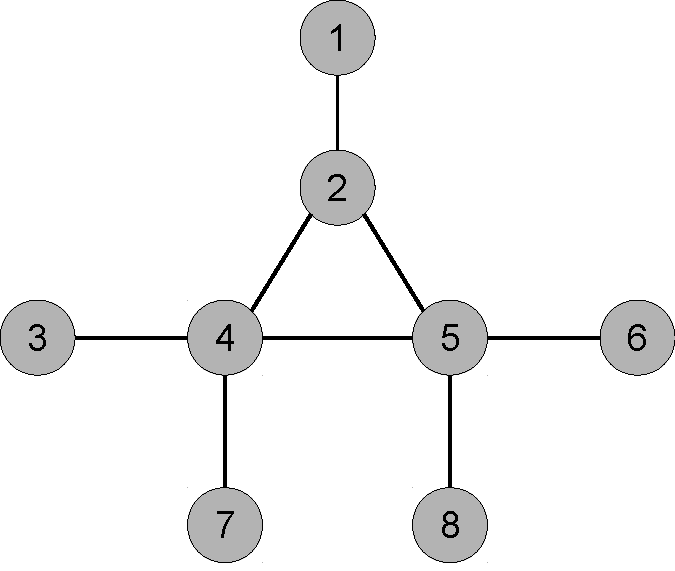
\includegraphics[scale=0.4]{graphe3}
\end{figure}

et définissons un algorithme pour déterminer s'il possède une
3-CLIQUE:

\begin{verbatim}
Possede-Une-3Clique(G):
  pour i := 1 à |G|-2:
    pour j := i+1 à |G|-1:
      pour k := j+1 à |G|:
        si (i, j, k) sont tous voisins:
          retourner vrai
        fin si
      fin pour
    fin pour
  fin pour
  retourner faux
fin
\end{verbatim}

L'algorithme trouvera qu'il existe une 3-CLIQUE entre les noeuds 2, 4
et 5.

Cet algorithme fonctionne en $O(n^3)$, clairement un temps polynomial.
Pour décider si un graphe possède une 4-CLIQUE, on ajouterait une
quatrième boucle dans le corps de l'algorithme et le temps d'exécution
serait $O(n^4)$.  Un algorithme décidant si un graphe possède une
$k$-CLIQUE pour un $k$ fixe fonctionnerait en $O(n^k)$, un temps
polynomial.

Donc, pour un $k$ fixe, décider si un graphe appartient à $k$-CLIQUE
se fait en temps polynomial, et ce langage appartient à P.


\end{document}






